\documentclass{beamer}

%%%%%%%%%%%%%%%%%%%%%%%%%%%%%%%%%%%%%%%%%%%%%%%%%%%%%%%%%%%%%%%%%%%%%%%%%%%%%%%%
% DEFINITIONS AND PACKAGES
%%%%%%%%%%%%%%%%%%%%%%%%%%%%%%%%%%%%%%%%%%%%%%%%%%%%%%%%%%%%%%%%%%%%%%%%%%%%%%%%

% Languages.
\usepackage[utf8]{inputenc}
\usepackage[english]{babel}
\usepackage[numberedbib]{apacite}
\usepackage{tikz}
\selectlanguage{english}

% Miscellaneous.
\usepackage{hyperref}

% Path to the figures directory.
\graphicspath{{figures/}}

%%%%%%%%%%%%%%%%%%%%%%%%%%%%%%%%%%%%%%%%%%%%%%%%%%%%%%%%%%%%%%%%%%%%%%%%%%%%%%%%
% TITLE SLIDE
%%%%%%%%%%%%%%%%%%%%%%%%%%%%%%%%%%%%%%%%%%%%%%%%%%%%%%%%%%%%%%%%%%%%%%%%%%%%%%%%

\title[A Computational Platform for Gene Expression Analysis]{A Computational Platform\\for Gene Expression Analysis}
\author[Diogo Teixeira]{
  Diogo Teixeira\inst{1}\\[1ex]
  {\footnotesize Supervisors: Rui Camacho\inst{2}, Nuno Fonseca\inst{3}}
}
\institute[FEUP]
{
  \inst{1}
  Check affiliation
  \and
  \inst{2}
  Check affiliation
  \and
  \inst{3}
  Check affiliation
}
\date{July 2014}
\subject{Informatics, Biology}

%%%%%%%%%%%%%%%%%%%%%%%%%%%%%%%%%%%%%%%%%%%%%%%%%%%%%%%%%%%%%%%%%%%%%%%%%%%%%%%%
% STYLE
%%%%%%%%%%%%%%%%%%%%%%%%%%%%%%%%%%%%%%%%%%%%%%%%%%%%%%%%%%%%%%%%%%%%%%%%%%%%%%%%

\makeatletter
\usetheme{Luebeck}
\usecolortheme{beaver}
\usefonttheme{serif}
\setbeamerfont{footline}{size=\fontsize{4}{12}\selectfont}
\setbeamertemplate{navigation symbols}{}
\setbeamertemplate{headline}{}
\setbeamertemplate{footline}
{%
  \leavevmode%
  \hbox{\begin{beamercolorbox}[wd=.23\paperwidth,ht=3.0ex,dp=2.0ex,center]{author in head/foot}%
      \usebeamerfont{author in head/foot}\insertshortauthor%
    \end{beamercolorbox}%
    \begin{beamercolorbox}[wd=.65\paperwidth,ht=3.0ex,dp=2.0ex,center]{title in head/foot}%
      \usebeamerfont{title in head/foot}\insertshorttitle
    \end{beamercolorbox}%
    \begin{beamercolorbox}[wd=.12\paperwidth,ht=3.0ex,dp=2.0ex,center]{author in head/foot}%
      \usebeamerfont{author in head/foot} \insertframenumber{} / \inserttotalframenumber
    \end{beamercolorbox}}%
  \vskip0pt
}

%%%%%%%%%%%%%%%%%%%%%%%%%%%%%%%%%%%%%%%%%%%%%%%%%%%%%%%%%%%%%%%%%%%%%%%%%%%%%%%%
% DOCUMENT
%%%%%%%%%%%%%%%%%%%%%%%%%%%%%%%%%%%%%%%%%%%%%%%%%%%%%%%%%%%%%%%%%%%%%%%%%%%%%%%%

\begin{document}

% Title slide.
\frame{\titlepage}

% TOC.
\begin{frame}
  \frametitle{Outline}
  \tableofcontents
\end{frame}

%%%%%%%%%%%%%%%%%%%%%%%%%%%%%%%%%%%%%%%%%%%%%%%%%%%%%%%%%%%%%%%%%%%%%%%%%%%%%%%%
% INTRODUCTION
%%%%%%%%%%%%%%%%%%%%%%%%%%%%%%%%%%%%%%%%%%%%%%%%%%%%%%%%%%%%%%%%%%%%%%%%%%%%%%%%

\section{Introduction}
\subsection{Domain Problem}
\begin{frame}[allowframebreaks]
  \frametitle{Domain Problem}
  \framesubtitle{Introduction}

\begin{itemize}
\item
Molecular biology is a young field of study, with a lot of unknowns and partial
knowledge.\\ \vspace{0.8cm}

\item
Studying gene expression is crucial to understand the mechanisms that control
living organisms.\\ \vspace{0.8cm}

\item
We focused on two different areas:
\begin{itemize}
  \item
  differential expression analysis;

  \item
  RNA-binding protein (RBP) discovery and analysis.
\end{itemize}
\end{itemize}

\framebreak

Three distinct problems:\\ \vspace{0.5cm}

\begin{itemize}
\item
Read alignment against a reference genome and differential expression analysis
on the aligned data.\\ \vspace{0.7cm}

\item
RBP discovery, analysis and information enrichment.\\ \vspace{0.7cm}

\item
Further result analysis using data mining techniques.

\end{itemize}

%NOTES:\\
%- Molecular biology is a new subject.\\
%- Many unknowns.\\
%- Gene expression is important...\\
%- Two areas of interest of IBMC experts: differential expression and RBPs.\\

\end{frame}

\subsection{Motivation and Objectives}
\begin{frame}
  \frametitle{Motivation and Objectives}
  \framesubtitle{Introduction}

\begin{columns}[<options>]
  \begin{column}{0.45\textwidth}
    \textcolor<5-6>{gray!40}{\textcolor<2-3>{gray!40}{\textbf{Tools are complex}\scriptsize\\
    Tools for biological data analysis often require a very technical set of
    skills.\\
    \vspace{0.8cm}}}

    \textcolor<6>{gray!40}{\uncover<2->{\textcolor<3-4>{gray!40}{\textbf{Tasks are repetitive}\scriptsize\\
    Analysing high quantities of data can be repetitive, especially if executed
    manually.\\
    \vspace{0.8cm}}}}

    \uncover<3->{\textcolor<4-5>{gray!40}{\textbf{Information is scattered}\scriptsize\\
    Information is easy to acquire, but is often scattered through multiple
    platforms, services and institutions.\\
    }}
  \end{column}

  \begin{column}{0.45\textwidth}
    \uncover<4-6>{\textcolor<5->{gray!40}{\textbf{Create simpler tools}\scriptsize\\
    Any user should be able to use the tools, with little to no training.\\
    \vspace{1.1cm}}}

    \uncover<5-6>{\textcolor<6->{gray!40}{\textbf{Automate tasks}\scriptsize\\
    Automated systems should perform repetitive tasks, so that users can
    focus on their work.\\
    \vspace{0.8cm}}}

    \uncover<6>{\textbf{Gather information}\scriptsize\\
    Information should be contextually aggregated, allowing for quick access of
    relevant information.
    }
  \end{column}
\end{columns}

%NOTES:\\
%Motivation:\\
%- Many tools require a very technical set of skills (tools should be facilitators, not hindrances)\\
%- Some tasks need automation.\\
%- Lots of information, often scattered in multiple places.\\
%Objectives:\\
%- Build simples tools that require minimal skill.\\
%- Automate processes.\\
%- Aggregate as much relevant information as possible.\\

\end{frame}

%%%%%%%%%%%%%%%%%%%%%%%%%%%%%%%%%%%%%%%%%%%%%%%%%%%%%%%%%%%%%%%%%%%%%%%%%%%%%%%%
% SOLUTION
%%%%%%%%%%%%%%%%%%%%%%%%%%%%%%%%%%%%%%%%%%%%%%%%%%%%%%%%%%%%%%%%%%%%%%%%%%%%%%%%

\section{Developed Solution}
\subsection{Overview}
\begin{frame}
  \frametitle{Overview}
  \framesubtitle{Developed Solution}

\begin{itemize}

\item
Two distinct problems warrant two different solutions.\\ \vspace{0.8cm}

\item
The developed system should be available anywhere, through the internet.\\ \vspace{0.8cm}

\item
The system's footprint should be small enough to allow deployment in almost any
available hardware.

\end{itemize}

%NOTES:\\
%- Two computer systems, one for each domain problem.\\
%- Both accessible through the web.\\
%- Focus on small system footprint, deployable by machine, department, institution.\\

\end{frame}

\subsection{RNA-Seq Analysis Pipeline}
\begin{frame}
  \frametitle{RNA-Seq Analysis Pipeline}
  \framesubtitle{Developed Solution}

NOTES:\\
- Show scheme, refer iRAP, the script and the web interface.\\
- Refer multiple differential expression tools.\\
- Refer user input and tool configuration.\\

\end{frame}

\subsection{RBP Analysis Pipeline (PBS Finder)}
\begin{frame}
  \frametitle{RBP Analysis Pipeline (PBS Finder)}
  \framesubtitle{Developed Solution}

NOTES:\\
- Show scheme, RBP finding, gene enrichment, clustering.\\
- Refer web interface.
- Refer that the tools is in production for several months, being extensively tested by experts.\\
- Refer user input and tool configuration.\\

\end{frame}

\subsection{Integration}
\begin{frame}
  \frametitle{Integration}
  \framesubtitle{Developed Solution}

\only<1>{
While focusing on aggregation and quick access to information, does it make
sense to separate the results into two different platforms?}

\only<1>{
\begin{figure}
  \centering
  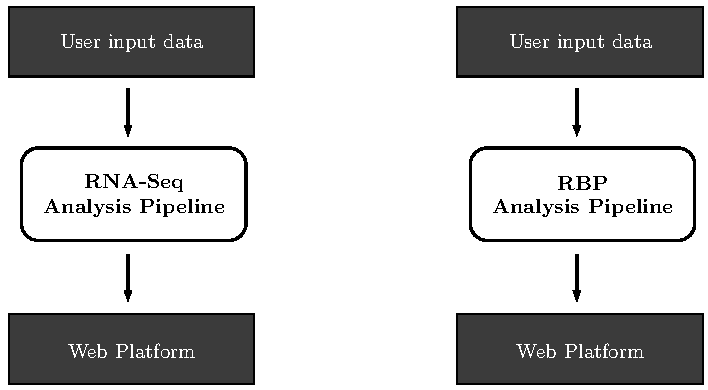
\includegraphics[width=0.8\textwidth]{integration1}
\end{figure}}

\only<2>{
A list of differentially expressed genes is not very useful without further
information about those genes. Does it make sense for a user to launch a new
gene enrichment task by hand?}

\only<2>{
\begin{figure}
  \centering
  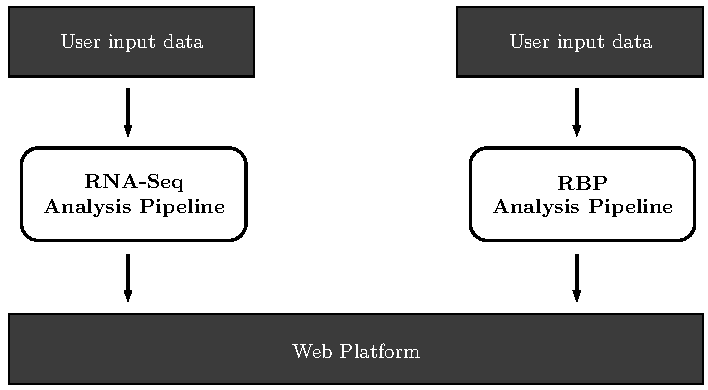
\includegraphics[width=0.8\textwidth]{integration2}
\end{figure}}

\only<3>{
A fully integrated solution: the analysis pipelines can be used separately or
automatically executed in sequence; result visualization for both pipelines is
isolated.}

\only<3>{
\begin{figure}
  \centering
  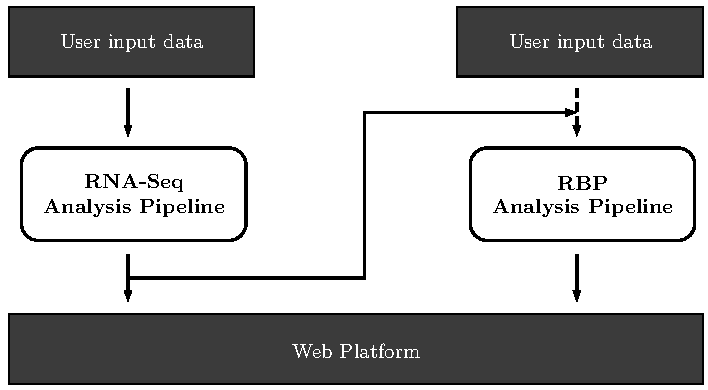
\includegraphics[width=0.8\textwidth]{integration3}
\end{figure}}

%NOTES:\\
%- Differential expression analysis could benefit from gene enrichment.\\
%- Do we really need two separate platforms?\\
%- Joined together, user choses what analysis to perform.\\
%- Still separate viewing experiences.\\

\end{frame}

%%%%%%%%%%%%%%%%%%%%%%%%%%%%%%%%%%%%%%%%%%%%%%%%%%%%%%%%%%%%%%%%%%%%%%%%%%%%%%%%
% CASE STUDIES
%%%%%%%%%%%%%%%%%%%%%%%%%%%%%%%%%%%%%%%%%%%%%%%%%%%%%%%%%%%%%%%%%%%%%%%%%%%%%%%%

\section{Case Studies}
\subsection{RNA-Seq Analysis Pipeline}
\begin{frame}
  \frametitle{RNA-Seq Analysis Pipeline}
  \framesubtitle{Case Studies}

NOTES:\\
- Refer objectives, data and experimental method.\\
- Refer results.\\

\end{frame}

\subsection{RBP Analysis Pipeline (PBS Finder)}
\begin{frame}
  \frametitle{RBP Analysis Pipeline (PBS Finder)}
  \framesubtitle{Case Studies}

NOTES:\\
- Refer objectives, data and experimental method.\\
- Refer results.\\
- Maybe show screenshot.\\

\end{frame}

%%%%%%%%%%%%%%%%%%%%%%%%%%%%%%%%%%%%%%%%%%%%%%%%%%%%%%%%%%%%%%%%%%%%%%%%%%%%%%%%
% CONCLUSIONS
%%%%%%%%%%%%%%%%%%%%%%%%%%%%%%%%%%%%%%%%%%%%%%%%%%%%%%%%%%%%%%%%%%%%%%%%%%%%%%%%

\section{Conclusions}
\subsection{Objective Fulfilment}
\begin{frame}
  \frametitle{Objective Fulfilment}
  \framesubtitle{Conclusions}

\begin{itemize}
\item
RBP analysis pipeline and web platform (PBS Finder) fully implemented. PBS
Finder has been in production for several months; during this time it was
thoroughly tested by IBMC experts.\\ \vspace{0.8cm}

\item
RNA-Seq analysis pipeline partially implemented (iRAP deployed and result
joining tool implemented).\\ \vspace{0.8cm}

\item
Integration of both tools could not be accomplished due to time constraints.
\end{itemize}

%NOTES:\\
%- All PBS Finder functionality implemented.\\
%- Differential expression analysis pipeline deployed, combination script created.\\
%- It was not possible to integrate with web platform, due to time constraints.\\

\end{frame}

\subsection{Future Work}
\begin{frame}
  \frametitle{Future Work}
  \framesubtitle{Conclusions}

\begin{itemize}
\item
Fully integrate the RNA-Seq analysis pipeline with the web platform (automatic
job configuration, result visualization, etc.).\\ \vspace{1.2cm}

\item
Study the requirements for deploying the platform in large scale, and assess the
feasibility of making it available internet-wide.
\end{itemize}

%NOTES:\\
%- Integrate the entire pipeline.\\
%- Study possibility of large scale deployment.\\

\end{frame}

%%%%%%%%%%%%%%%%%%%%%%%%%%%%%%%%%%%%%%%%%%%%%%%%%%%%%%%%%%%%%%%%%%%%%%%%%%%%%%%%
% DOCUMENT END
%%%%%%%%%%%%%%%%%%%%%%%%%%%%%%%%%%%%%%%%%%%%%%%%%%%%%%%%%%%%%%%%%%%%%%%%%%%%%%%%

% TOC.
\begin{frame}
  \frametitle{Review}
  \tableofcontents
\end{frame}

% TODO
% Remove if no references.
%\begin{frame}{Bibliography}
  %\bibliographystyle{apacite}
  %\bibliography{myrefs}
%\end{frame}

% Title slide.
\frame{\titlepage}

\end{document}
